\documentclass{article}
\usepackage{graphicx} % Required for inserting images
\usepackage{booktabs} % Required for inserting summary table
\usepackage{float}
\usepackage[margin=1in]{geometry}
\usepackage{hyperref}
\hypersetup{hidelinks}

\begin{document}

\begin{titlepage}

\centering
\vspace*{2in}
{\Huge\bfseries Final Project\par}
\vspace{0.5cm}
{\large COL1A1 Expression in TCGA Breast Invasive Carcinoma\par}
\vspace{2cm}
{\large Steven Hutchins, MBA\par}
\vspace{0.3cm}
{\large HSE 711: Foundations in Data Science\par}
{\large Geisel School of Medicine at Dartmouth\par}
\vspace{0.3cm}
{\large October 2026\par}
\end{titlepage}

\tableofcontents
\newpage

\section{Introduction}

\subsection{Data Description}
The data for this analysis were provided by the course instructor via Canvas as two files: a matrix of RNA-sequencing raw gene counts and a sample metadata file. The data originate from the Cancer Genome Atlas Breast Invasive Carcinoma Project (TCGA-BRCA)~\cite{TCGA2012BRCA, Grossman2016GDC}. The count matrix contains RNA-sequencing raw gene counts for 60,660 genes across 1,231 samples. Each sample is identified by its TCGA barcode and classified by sample type as primary solid tumor, solid tissue normal, or metastatic. Sequencing depth varied widely across samples, from about 19 to 114 million total reads (median about 58 million). Counts were not normalized for library size, so comparisons between samples are approximate.

\subsection{Biological Relevance of COL1A1}
COL1A1 is a collagen gene. It encodes the alpha-1 chain of type I collagen, the most abundant structural protein in the human body and the main component of the extracellular matrix that supports tissues, including the breast. In breast cancer, the tissue surrounding a tumor often becomes dense and fibrotic as excess collagen is produced. This collagen-rich environment stiffens the tissue and has been linked to tumor invasion, metastasis, and worse patient outcomes~\cite{Liu2018COL1A1, Provenzano2008, Levental2009, Conklin2011}.

\section{Methods}

\subsection{Software and Packages}
All analyses were performed in R (version 4.6.1) using RStudio and R Markdown. Data wrangling used the \texttt{tidyverse} (2.0.0), mainly \texttt{dplyr} (1.2.1) for filtering, selecting, and summarizing and \texttt{tidyr} (1.3.2) for reshaping data between wide and long formats. The histogram, scatter plot, violin plot, and mean-difference plot were made with \texttt{ggplot2} (4.0.3), with axis labels formatted by \texttt{scales} (1.4.0). The heatmap was made with Bioconductor package \texttt{ComplexHeatmap} (2.28.0). Summary statistics (n, mean, median, standard deviation, minimum and maximum) were calculated with a custom function using base R and exported as a LaTeX table with \texttt{knitr} (1.52). Figures were saved as PDFs with \texttt{ggsave} and the base R \texttt{pdf()} device. The final report was written in LaTeX using Overleaf.

\subsection{Primary Gene Selection}
To select my primary gene of interest, I calculated each gene's mean raw count separately in tumor and normal samples and took the difference between them (tumor minus normal). Ranking genes by the size of this difference, COL1A1 (ENSG00000108821.14) had the largest gap with a mean of about 412,800 counts in tumor samples compared with 84,700 in normal samples. For this reason, I selected it as my primary gene for this analysis.

\subsection{Secondary Gene Selection}
FN1 was selected as the secondary gene using the same approach as COL1A1. Ranked by the absolute difference in mean raw counts between tumor and normal samples, FN1 (ENSG00000115414.21) had the second-largest gap, with a mean of about 311,700 counts in tumor tissue compared with 39,900 in normal tissue. FN1 encodes fibronectin, a major extracellular matrix protein. Like type I collagen, fibronectin is produced largely by fibroblasts.

\subsection{Random Gene Selections}
To give context for the targeted selection of primary and secondary genes, ten additional genes were drawn at random from the full dataset using a fixed seed (777) for reproducibility. These genes were not chosen for any known link to breast cancer. They provide a baseline view of how a typical gene is represented in this dataset.

Comparing the two approaches shows what each one does well. The targeted strategy picked out genes with large tumor-normal differences and clear biological relevance, which led directly to meaningful patterns: high COL1A1 expression in tumors and a strong link between COL1A1 and FN1. The random sample, by contrast, showed that most genes are expressed at low levels, vary little between samples, and do not separate tumor from normal tissue. Several of the randomly selected genes are not even annotated with a gene symbol. Together, these results show that the changes seen in COL1A1 and FN1 are not typical in the dataset as a whole. A random sample does avoid the selection bias built into the targeted approach, but it is unlikely to reveal disease-relevant biology on its own. The two methods together give both a focused signal and a reference point for judging how unusual that signal is.

\section{Results}

\subsection{Summary Statistics}
\begin{table}[H]

\caption{\label{tab:unnamed-chunk-9}Summary statistics for COL1A1 and FN1 raw counts}
\centering
\begin{tabular}[t]{llrrrrrr}
\toprule
gene\_symbol & tcga\_barcode & n & mean & median & sd & min & max\\
\midrule
COL1A1 & ENSG00000108821.14 & 1,231 & 381,894.4 & 270,257 & 378,083.3 & 1,329 & 3,257,937\\
FN1 & ENSG00000115414.21 & 1,231 & 285,915.9 & 190,342 & 303,893.9 & 1,572 & 2,465,891\\
\bottomrule
\end{tabular}
\end{table}


\subsection{Histogram}
\begin{figure}[H]
    \centering
    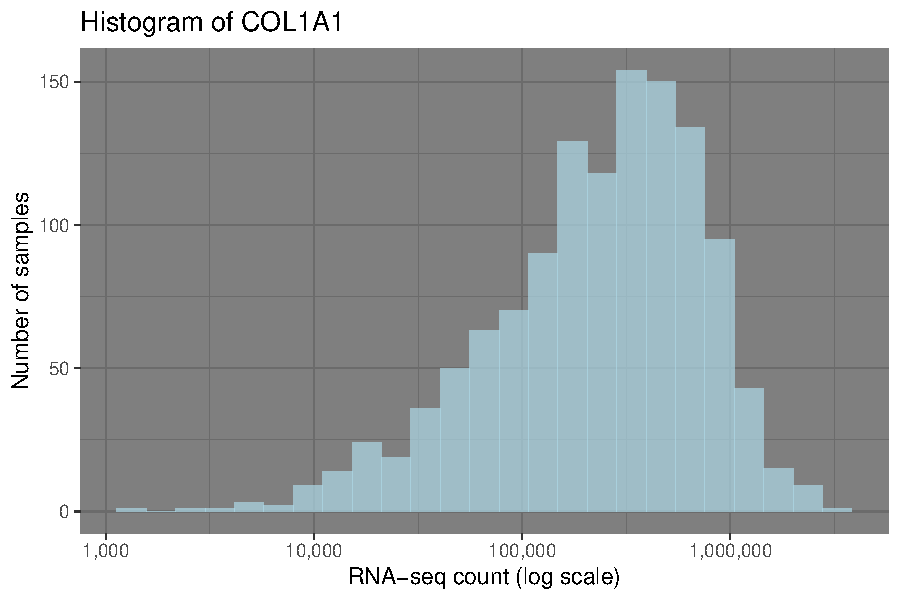
\includegraphics[width=0.85\textwidth]{histogram.pdf}
    \caption{Distribution of COL1A1 raw counts across 1,231 samples, shown on a log10 scale.}
    \label{fig:histogram}
\end{figure}
Figure~\ref{fig:histogram} shows how COL1A1 raw counts are distributed across all 1,231 samples, with counts on a log10 scale. Expression is high in most samples. The distribution peaks between roughly 200,000 and 600,000 counts, and the median is 270,257. The distribution is left-skewed on a log scale: a long tail stretches down toward 1,000 to 10,000 counts, while the right side drops off quickly above 1,000,000. Counts span more than three orders of magnitude, from 1,329 to 3,257,937, which is why a log scale was needed to show the full range.

This spread likely reflects a mix of sample types in the dataset. Most samples are primary tumors, where COL1A1 tends to be highly expressed, so they probably make up the main peak. The lower tail may include normal tissue samples or tumors with less collagen-rich stroma, though the histogram alone can't confirm this. The violin plot by sample type addresses that question directly. Some of the spread may also come from differences in sequencing depth, since the counts were not normalized. 

\subsection{Scatter Plot}
\begin{figure}[H]
    \centering
    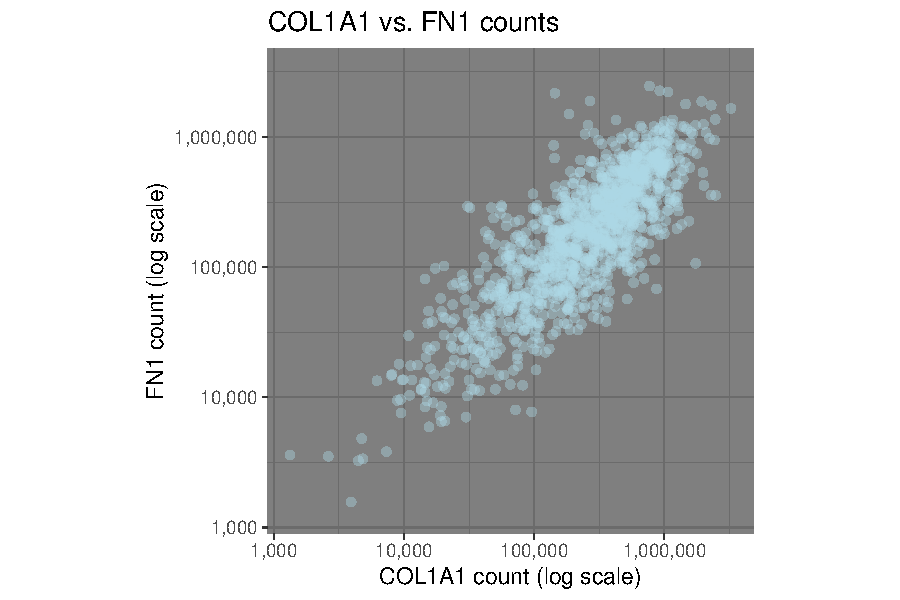
\includegraphics[width=0.85\textwidth]{scatter_plot.pdf}
    \caption{COL1A1 versus FN1 raw counts for each sample, both on log10 scales}
    \label{fig:scatter}
\end{figure}
Figure~\ref{fig:scatter} compares COL1A1 and FN1 raw counts for each of the 1,231 samples, with both axes on a log10 scale. The two genes show a strong positive relationship. Samples with high COL1A1 expression almost always have high FN1 expression too, and the points form a tight diagonal band running from the lower left to the upper right. Most samples cluster in the upper right, between about 100,000 and 1,000,000 counts for both genes, which matches the high expression seen in the histogram. A smaller group of samples sits at lower counts for both genes, roughly 1,000 to 30,000.

This pattern makes biological sense. FN1 encodes fibronectin, another major extracellular matrix protein, and, like type I collagen, it is produced primarily by fibroblasts in the tissue surrounding a tumor. Because the two genes are made by the same cells and serve related structural functions, samples with more stromal or fibrotic tissue are expected to have higher levels of both. The relationship could also be partly influenced by differences in sequencing depth: a deeply sequenced sample will show higher counts of both genes at once, so normalization would be needed to confirm how much of the correlation is biological. No correlation coefficient was calculated, so this relationship is described visually rather than statistically.

\subsection{Violin Plot}
\begin{figure}[H]
    \centering
    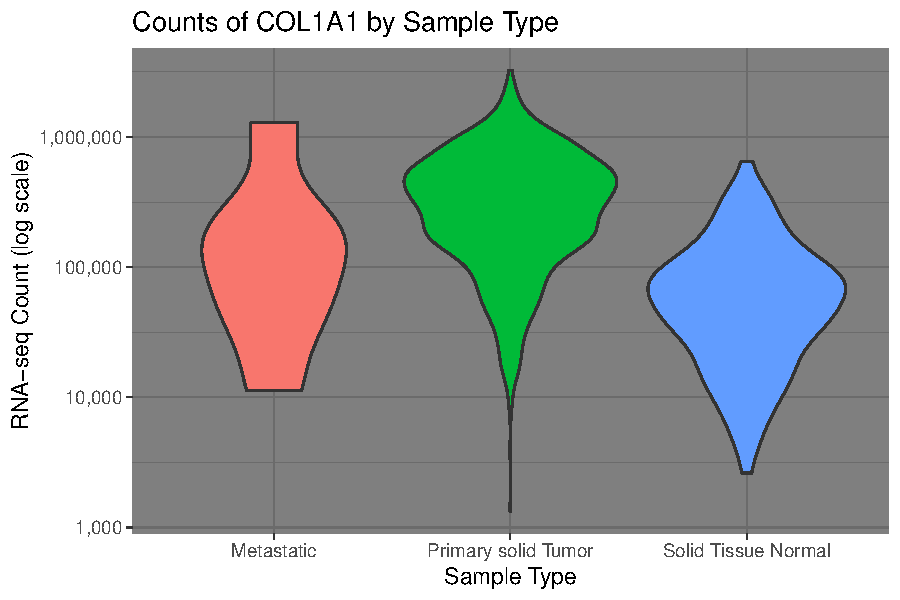
\includegraphics[width=0.85\textwidth]{violin.pdf}
    \caption{COL1A1 raw counts by sample type (metastatic, primary solid tumor, and solid tissue normal), shown on a log10 scale}
    \label{fig:violin}
\end{figure}
Figure~\ref{fig:violin} shows the distribution of COL1A1 raw counts across three sample types: 1,111 primary solid tumors, 113 solid tissue normal samples, and 7 metastatic samples. Counts are on a log10 scale, and the width of each violin shows how many samples fall at each expression level. Primary solid tumors have the highest typical expression, concentrated between roughly 200,000 and 600,000 counts, with a long lower tail. Solid tissue normal samples are centered noticeably lower, around 50,000 to 100,000 counts. The metastatic group falls in between and is spread widely, but with only 7 samples its shape is not reliable and should be interpreted with caution.

The higher COL1A1 expression in primary tumors compared with normal tissue matches the tumor-normal gap that led to selecting this gene. It also fits the known roles of collagen-rich, fibrotic tissue around breast tumors. The groups overlap somewhat, but the lower tail of the tumor distribution extends into the range of normal samples, so COL1A1 alone would therefore not perfectly separate tumor from normal samples. The groups are also very unequal in size, with tumors making up about 90\% of the dataset. As with the other figures, the counts are not normalized for sequencing depth.

\subsection{Heatmap}
\begin{figure}[H]
    \centering
    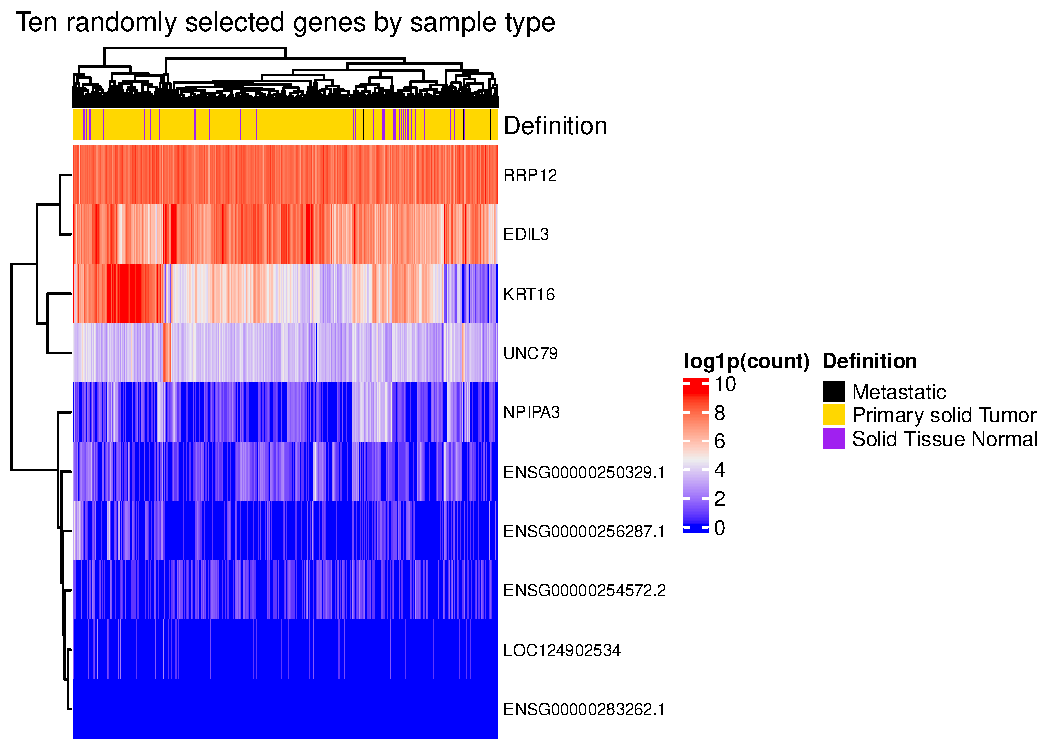
\includegraphics[width=0.85\textwidth]{heatmap.pdf}
    \caption{Heatmap of log1p-transformed counts for ten randomly selected genes (seed 777), with samples grouped by sample type. Genes without an annotated symbol are labeled by their Ensembl ID.}
    \label{fig:heatmap}
\end{figure}
Figure~\ref{fig:heatmap} shows log1p-transformed counts for ten randomly selected genes (seed 777) across all samples, with sample type shown in the annotation bar along the top. Rows and columns were clustered so that genes and samples with similar expression patterns appear next to each other. The genes fall into two broad groups. RRP12, EDIL3, KRT16, and UNC79 have moderate to high expression in most samples, while NPIPA3, LOC124902534, and the unannotated genes have low expression throughout. KRT16, a keratin gene found in epithelial cells, shows the most variation between samples: it is strongly expressed in one cluster of samples and much lower in others.

Because these genes were chosen at random rather than for a known link to breast cancer, the heatmap mainly shows general expression patterns in the dataset rather than tumor-specific changes. Most randomly chosen genes are expressed at low levels, which is common in RNA-seq data. Samples do not separate clearly by type in the clustering, which suggests that these ten genes on their own do not distinguish tumor from normal tissue. Several of the selected genes have no annotated gene symbol and are labeled by their Ensembl ID.

\subsection{Mean-Difference Plot}
\begin{figure}[H]
    \centering
    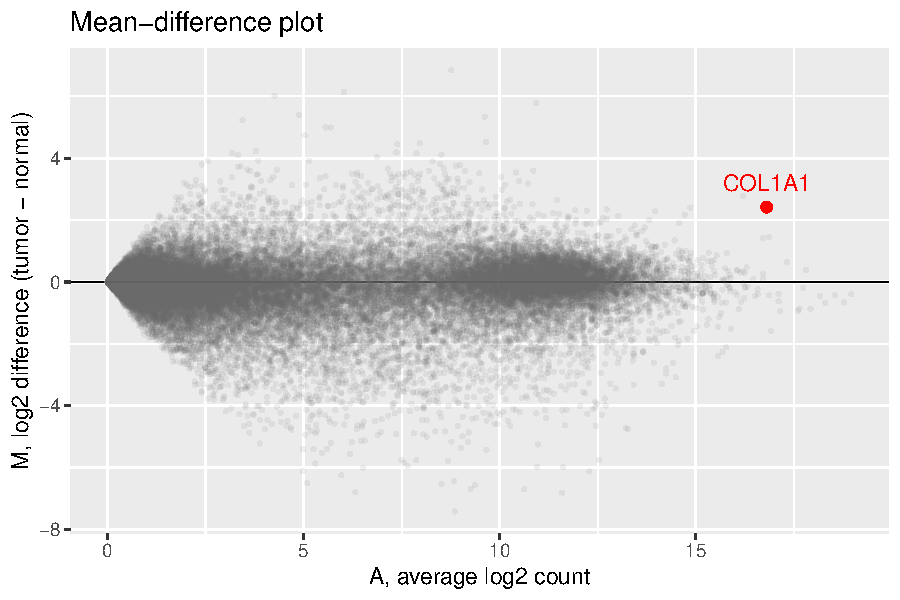
\includegraphics[width=0.85\textwidth]{ma_plot.pdf}
    \caption{Mean-difference (MA) plot of tumor versus normal expression for all genes. M is the difference in mean log2 count (tumor minus normal), and A is the average of the two. COL1A1 is highlighted in red.}
    \label{fig:mean_diff}
\end{figure}
Figure~\ref{fig:mean_diff} compares tumor and normal expression for every gene in the dataset. The x-axis (A) is each gene's average log2 count across the two groups, and the y-axis (M) is the difference in mean log2 count between tumor and normal samples. Points above zero are more highly expressed in tumors and points below zero are more highly expressed in normal samples. The spread in M is widest at low average expression and narrows as expression increases. This funnel shape is typical because low counts are noisier, so small absolute changes produce large log differences.

COL1A1, highlighted in red, stands out in the upper right. It is one of the most highly expressed genes in the dataset (A of about 17) and has an M of about 2.4, meaning its average log2 expression is roughly 2.4 units higher in tumors, or about five-fold higher. Few genes at this expression level show a tumor-normal difference this large, which supports its selection as the primary gene. The cloud of points is centered near zero, which suggests that differences in sequencing depth did not strongly bias the overall comparison. However, the counts were not normalized for library size, so the M values should be treated as approximate. A formal differential expression analysis with dedicated tools such as \texttt{DESeq2} or \texttt{edgeR} would be needed to confirm these differences statistically.

\subsection{Trends and Interpretation}
Across all analyses, the clearest pattern is that COL1A1 is expressed at higher levels in breast tumors than in normal breast tissue. The violin plot shows primary tumors centered well above normal samples, and the mean-difference plot places COL1A1 among the most highly-expressed genes with one of the largest tumor-normal differences in the dataset. FN1 shows a similar pattern and rises closely with COL1A1 across samples, as seen in the scatter plot. Because both genes encode major extracellular matrix proteins produced largely by fibroblasts, their shared increase is consistent with dense, collagen-rich tissue known to surround many breast tumors.

The randomly selected genes provide useful contrast. Most were expressed at low levels, varied little, and did not separate tumor from normal samples, which suggests the large differences seen in COL1A1 and FN1 are not typical of the dataset as a whole. At the same time, the overlap between tumor and normal samples in the violin plot shows that COL1A1 alone would not reliably distinguish cancerous from healthy tissue.

These findings come with several limitations. Counts were not normalized for sequencing depth, which varied nearly sixfold across samples, so all comparisons are approximate. No formal statistical tests or correlation coefficients were calculated, the sample groups were very unequal in size, and the metastatic group contained only seven samples. A more rigorous follow-up would normalize the counts, test for differential expression with tools such as \texttt{DESeq2} or \texttt{edgeR} and quantify the relationship between COL1A1 and FN1.

\addcontentsline{toc}{section}{References}

\bibliographystyle{unsrt}
\bibliography{refs}
\end{document}
